\documentclass[11pt]{article}

\usepackage[utf8]{inputenc}
\usepackage[margin=1cm]{geometry}
\usepackage{polski}
\usepackage{titling}
\usepackage{romannum}
\usepackage{amsmath}
\usepackage{amssymb}
\usepackage{amsthm}
\usepackage{mathdots}
\usepackage{fullpage}
\usepackage{gensymb}
\usepackage{MnSymbol}
\usepackage{stmaryrd}
\usepackage{graphicx}
\usepackage{subcaption}
\usepackage{multirow}
\usepackage{dsfont}
\usepackage{url}

\def\R{\mathbb{R}}
\def\C{\mathbb{C}}
\def\Z{\mathbb{Z}}
\def\Q{\mathbb{Q}}
\def\N{\mathbb{N}}
\def\Rn{\mathbb{R}^n}
\def\E{\mathcal{E}}
\def\B{\mathcal{B}}
\def\1{\mathds{1}}
\def\nor{\trianglelefteq}
\def\ker{\operatorname{ker}}
\def\gengru#1{\langle\,#1 \,\rangle}
\def\ch{\blacktriangleleft}
\def\arr{\longrightarrow}
\def\Abs#1{\left\vert#1\right\vert}
\def\rk{\operatorname{rank}}
\def\lin{\operatorname{lin}}
\def\af{\operatorname{af}}
\def\dim{\operatorname{dim}}
\def\ker{\operatorname{ker}}
\def\im{\operatorname{im}}
\def\tr{\operatorname{tr}}
\def\Hom{\operatorname{Hom}}
\def\Aut{\operatorname{Aut}}
\def\id{\triangleleft}
\def\iif{\operatorname{if}}
\newcommand{\norm}[1]{\left\lVert#1\right\rVert}
\def\normsign{\|\cdot\|}
\newcommand{\series}[3]{\sum_{#1}^{#2}#3}

\newtheorem{problem}{Problem}
\newtheorem{definicja}{Definicja}

\setlength{\droptitle}{-2cm}
\title{Optymalna strategia podawania leku}
\author{Tomasz Kanas}

\begin{document}
\pagenumbering{gobble}
\maketitle

\section{Sformułowanie problemu}
Celem pracy jest znalezienie strategii podawania leku, przy leczeniu nowotworu, pozwalającej osiągnąć możliwie największą skuteczność terapii. W tym celu skorzystamy z modelu przedstawionego w pracy \cite{BBF-manuscript}. Model ten przedstawia rozwój nowotworu w czasie w zależności od dawkowania leku za pomocą równania różniczkowego:
\begin{equation} \label{ode}
  \begin{aligned} 
    V_1'(t) &= \lambda_1V_1F\left(\frac{V_1 + \alpha_{12}V_2}{K}\right) - \beta_1V_1g(t), \\
    V_2'(t) &= \lambda_2V_2F\left(\frac{V_2 + \alpha_{21}V_1}{K}\right) - \beta_2V_2g(t), \\
    K'(t) &= -\mu K + (V_1+V_2) - d{(V_1 + V_2)}^{2/3}K - \beta K g(t) \\
  \end{aligned}
\end{equation}
dla $t \in [0, T]$, z warunkami początkowymi
\begin{equation} \label{ode-start}
   V_1(0) = V_{10},\ V_2(0) = V_{20},\ K(0) = K_0
\end{equation}
gdzie $F(x) = -\ln(x)$, $ 0 \le g(t) \le g_{\max}$, oraz
\[\lambda_1, \lambda_2, \alpha_{12}, \alpha_{21}, \beta_1, \beta_2, \beta, \mu, d, V_{10}, V_{20}, K_0 \ge 0\]
są zadanymi parametrami.

Funkcja $V_1(t)$ modeluje liczbę komórek guza podatnych na lek w momencie $t$, $V_2(t)$ liczbę komórek guza odpornych na lek, a $K(t)$ jest parametrem nazwanym w pracy ,,unaczynieniem''. Zauważmy, że rozwiązania $V_1, V_2, K$ zależą od wyboru funkcji $g$ którą nazywamy sterowaniem. W tym modelu wartość $g(t)$ ma interpretację jako wielkość dawki leku w czasie $t$.

Zadanie polega na znalezieniu funkcji $g: [0, T] \to [0, g_{\max}]$ oraz $V_1, V_2, K: [0, T] \to (0, \infty)$ spełniających (\ref{ode}), oraz minimalizujących funkcjonał:
\begin{equation} \label{objf}
  J(g, V_1, V_2, K) = \int_0^T V_1(t) + V_2(t)dt + \omega\int_0^T G\left(\frac{V_2(t) - V_1(t)}{\epsilon}\right) dt
\end{equation}
gdzie
\begin{equation*}
  G(x) = \frac{1+\tanh(x)}{2} \quad
  \omega, \epsilon > 0 
\end{equation*}

Problem ten w literaturze nazywa się problemem optymalnego sterowania.

\subsection{Problem wyjściowy}
Zdefiniujmy teraz formalnie problem oraz uprościmy notację.

\begin{problem}\label{problem}
  Znaleźć funkcję kawałkami ciągłą
  \[g: [0, T] \to [0, g_{\max}]\]
  i funkcję
  \[y = {(y_1, y_2, y_3)}^T: [0,T] \to {(0, \infty)}^3\]
  spełniające równanie różniczkowe:
  \begin{equation}\label{odesim}
    \begin{aligned}
      \dot{y}(t) &= f(t, y, g) \\
      y(0) &= y_0 = {(y_{10}, y_{20}, y_{30})}^T
    \end{aligned}
  \end{equation}
  oraz minimalizujące funkcjonał
  \begin{equation}\label{objfsim}
    J(g, y) = \int_0^T y_1(t) + y_2(t)dt + \omega\int_0^T G\left(\frac{y_2(t) - y_1(t)}{\epsilon}\right) dt
  \end{equation}
  gdzie $f = {(f_1, f_2, f_3)}^T$ jest określone wzorem
  \begin{equation}\label{dynamicsim}
    \begin{aligned}
      f_1(t, y, g) &= \lambda_1y_1F\left(\frac{y_1 + \alpha_{12}y_2}{y_3}\right) - \beta_1y_1g(t), \\
      f_2(t, y, g) &= \lambda_2y_2F\left(\frac{y_2 + \alpha_{21}y_1}{y_3}\right) - \beta_2y_2g(t), \\
      f_3(t, y, g) &= -\mu y_3 + (y_1+y_2) - d{(y_1 + y_2)}^{2/3}y_3 - \beta y_3 g(t) \\
    \end{aligned}
  \end{equation}
\end{problem}

Przez funkcję kawałkami ciągłą określoną na odcinku rozumiemy funkcję o skończonej liczbie punktów nieciągłości. Jako, że o funkcji $f$ zakładamy tylko kawałkami ciągłość, należy doprecyzować co rozumiemy przez (\ref{odesim}). Załóżmy, że punktami nieciągłości $f$ są $\xi_1,\ \ldots,\ \xi_n$, wtedy (\ref{odesim}) oznacza ciąg równań różniczkowych postaci
\begin{equation}\label{nonconode}
  \begin{aligned}
    \dot{y}|_{(\xi_i, \xi_{i+1})}(t) &= f|_{(\xi_i, \xi_{i+1})}(t, y, g)\\
    y(\xi_i) &= \lim_{t\to \xi_i^-}y(t)
  \end{aligned}
  \quad \text{ gdzie } i \in \{0,\ldots, n\},\ \xi_0 = 0,\ \xi_{n+1}=T
\end{equation}

Zwróćmy jeszcze uwagę na fakt, że funkcja $F(x) = -\ln(x)$ posiada osobliwość w 0, więc prawa strona (\ref{dynamicsim}) nie jest dobrze zdefiniowana dla $y_1(t) = y_2(t) = 0$, a obliczenia w których argumenty $F$ są bliskie 0 mogą być obarczone dużymi błędami numerycznymi. Podobnie we wzorze (\ref{dynamicsim}) występuje dzielenie przez $y_3$, więc dla $y_3(t) = 0$ prawa strona (\ref{odesim}) także nie jest dobrze określone.

\subsection{Problem przybliżony}
Wyznaczenie rozwiązania problemu optymalnego sterowania w postaci jawnego wzoru rzadko kiedy jest możliwe. Z tego powodu zdecydujemy się na szukanie rozwiązania przybliżonego.

Rozwiązanie problemu \ref{problem} przybliżymy rozwiązaniem pewnego problemu optymalizacji skończenie wymiarowej. W tym celu ustalimy siatkę dyskretyzacji przedziału $[0, T]$:
\begin{equation}
  0 = t_0 < t_1 < \cdots < t_{n-1} < t_n = T
\end{equation}
Możemy teraz przybliżać sterowanie $g$ za pomocą splajnu opartego na punktach $t_{i}$. Dla prostoty ograniczymy się do splajnów stopnia 0 i 1. Ostatecznie przybliżone sterowanie $\hat{g}$ ma postać:
\begin{gather}  
    \hat{g}(t) = g_i \text{ gdy } t \in [t_{i}, t_{i + 1}) \label{control_1}\\
    \nonumber \text{lub} \\
    \hat{g}(t) = \frac{(t_{i+1} - t)g_i + (t - t_i)g_{i+1}}{t_{i+1} - t_i} \text{ gdy } t \in [t_i, t_{i+1}) \label{control_2}
\end{gather}
i jest jednoznacznie zdefiniowane przez wartości $g_i$ dla $i = 0,\ldots, n$. Te wartości będą optymalizowanymi zmiennymi.

Korzystając z przybliżonej funkcji sterowania, przybliżymy rozwiązanie $y$ równania różniczkowego (\ref{odesim}). Użyjemy do tego metody Rungego-Kutty rzędu $r$ ze stałym krokiem długości $h$, wtedy przybliżone rozwiązanie $\hat{y}(t) \simeq y(t)$ w punkcie $t = t_n + (m + 1)h$ dla $m = 0,\ldots, \frac{t_{n+1}-t_n}{h} - 1$  wyraża się przez:
\begin{equation} \label{rk}
  \begin{split}
    &k_1 = f(t_n + mh, \hat{y}(t_n + mh), \hat{g}) \\
    &k_l = f(t_n + c_l h, \hat{y}(t_n + mh) + h \sum_{i = 1}^{l-1} a_{li}k_i, \hat{g}) \\
    &\hat{y}(t_n + (m+1)h) = \hat{y}(t_n + mh) + h \sum_{i = 1}^r b_i k_i
  \end{split}
\end{equation}
gdzie $c_l, a_{li}, b_i$ są stałymi zależnymi od wybranej metody.

Zostało już tylko przybliżyć funkcjonał celu (\ref{objfsim}). Zapiszmy go w postaci
\begin{equation} \label{objf-sim}
  J(y) = \int_0^T j(y(t)) dt
\end{equation}
gdzie
\begin{equation}
  j(y) = y_1 + y_2 + \omega G\left(\frac{y_2 - y_1}{\epsilon} \right)
\end{equation}
wtedy ogólny wzór na kwadraturę ze stałym krokiem $h$ przybliżającą (\ref{objf-sim}) to
\begin{equation} \label{quad}
  Q(\hat{y}) = h\sum_{i = 0}^N \alpha_i j(\hat{y}(ih))
\end{equation}
gdzie $N = \frac{T}{h}$, a $\alpha_i$ są stałymi zależnymi od wybranej kwadratury.

Zatem możemy zdefiniować przybliżoną funkcję celu jako funkcję $g_1,\ldots,g_n$:
\begin{equation}
  \hat{J}(g_1,\ldots, g_n) = Q(\hat{y})
\end{equation}
ponieważ $\hat{y}$ jest jednoznacznie wyznaczony przez $\hat{g}$ za pomocą (\ref{rk}), a $\hat{g}$ jest wyznaczone jednoznacznie przez $g_1,\ldots,g_n$. Podsumowując, problem przybliżony to:
\begin{problem}\label{problemapprox}
  Znaleźć $g_1,\ldots, g_n$ minimalizujące
\begin{equation}\label{nlp}
  \hat{J}(g_1,\ldots, g_n)
\end{equation}
i spełniające
\begin{equation}\label{nlp_cons}
  \forall_{i \in \{1,\ldots,n\}} 0 \le g_i \le g_{\max}
\end{equation}
\end{problem}

Jest to problem optymalizacji nieliniowej z ograniczeniami i istnieją implementacje metod pozwalających uzyskać przybliżone rozwiązanie tego problemu. To podejście do numerycznego problemu optymalnego nazywa się ,,direct single shooting'' i występuje np. w~\cite{diehl} i~\cite{rao-methods}.

\subsection{Alternatywne podejście}

Innym popularnym podejściem jest ,,direct collocation''. W tym podejściu zaczyna się tak samo od dyskretyzacji czasu:
\[0 = t_0 < t_1 < \ldots < t_n = T\]
Następnie zarówno sterowanie jak i stan układu przybliża się splajnem opartym na punktach $t_i$. Dzięki temu sterowanie jest jednoznacznie wyznaczone przez wartości $g_i = \hat{g}(t_i)$, natomiast stan ukłądu przez wartości $y_i = \hat{y}(t_i)$. Celem jest, tak samo jak w powyższym podejściu, sprowadzenie problemu do problemu optymalizacji nieliniowej z ograniczeniami. Aby móc to zrobić należy znaleźć warunki jakie wartości $y_i$ muszą spełniać, aby układ spełniał w przybliżeniu równanie
\[\dot{y}(t) = f(t,y(t),g(t))\]
Aby znaleźć te warunki przybliża się całkę z powyższego równania za pomocą pewnej kwadratury. Dla przykładu ustalmy kwadraturę trapezową. Wtedy dostajemy równanie przybliżone
\[\int_{t_i}^{t_{i+1}} \dot{y}(t)dt = \int_{t_i}^{t_{i+1}} f(t,y(t),g(t))dt\]
\[y_{i+1} - y_{i} \simeq \frac{1}{2}(t_{i+1}-t_i)(f(t_{i+1}, y_{i+1}, g(t_{i+1})) - f(t_i, y_i, g(t_i)))\]
Ograniczenia występujące w sformułowaniu oryginalnego problemu można zwykle bez problemu przekształcić na ograniczenia na $g_i$ oraz $y_i$. Można też zdefiniować przybliżony funkcjonał celu jako numeryczne przybliżenie oryginalnego funkcjonału celu zastosowane do przybliżonego stanu $\hat{y}$.
% TODO

Podejście to jest dokładnie opisane w \cite{Kelly}, występuje też w \cite{diehl} i \cite{rao-methods}.

\subsection{Plan rozwiązania}
Aby obliczyć wynik problemu przybliżonego skorzystamy ze środowiska MATLAB/Octave wraz z dostarczonym z nim optymalizatorem problemu optymalizacji nieliniowej z ograniczeniami (FMINICON). W tym celu zaimplementujemy przejście od problemu optymalnego sterowania. Aby poprawić złożoność czasową optymalizacji i tym samym umożliwić stosowanie gęstszej siatki dyskretyzacji, obliczymy gradient przybliżonej funkcji celu. Będziemy też musieli znaleźć odpowiednią siatkę dyskretyzacji i punkt startowy dla optymalizatora.

\section{Implementacja}
Optymalizator FMINICON wymaga dostarczenia funkcji do optymalizowania, czyli w naszym przypadku funkcji $\hat{J}$, oraz ograniczeń, czyli w naszym przypadku jedynie (\ref{nlp_cons}). Domyślnie optymalizator wyznacza gradient za pomocą różnic skończonych, co wymaga uruchomienia funkcji celu liniowo wiele razy względem liczby parametrów. Aby poprawić wydajność optymalizacji zaimplementujemy liczenie gradientu przybliżonej funkcji celu ze względu na parametry $g_1,\ldots, g_n$.

Zauważmy, że znalezienie dobrego wyniku będzie wymagało zapewne wielokrotnego wywołania naszej funkcji celu przez optymalizator, więc zależy nam aby funkcja celu liczyła się możliwie szybko. Lepsza wydajnościowo implementacja pozwoli też na większe zagęszczenie siatki dyskretyzacji i tym samym wzrost dokładności aproksymacji.

Jedną z praktyk pozwalającą poprawić wydajność programów w środowiskach MATLAB i Octave jest tak zwana wektoryzacja. Polega ona na zastępowaniu pętli operacjami na wektorach. Korzysta to z faktu, że wiele funkcji w tych środowiskach można wywołać z wektorem parametrów, zamiast pojedynczego parametru i zwracają one wtedy wektor wyników, oraz wykonują się znacznie szybciej niż gdyby wywołać je wielokrotnie w pętli. Z tego powodu będziemy korzystać z tej techniki gdzie to tylko możliwe.

Aby sprowadzić problem optymalnego sterowania do problemu optymalizacji nieliniowej musimy obliczyć przybliżone sterowanie (\ref{control_1}) lub (\ref{control_2}), przybliżyć rozwiązanie równania różniczkowego (\ref{rk}) a następnie za pomocą uzyskanego rozwiązania obliczyć kwadraturę (\ref{quad}) przybliżającą funkcję celu (\ref{objf}). Ponadto chcemy obliczyć gradient funkcji celu, co będzie wymagało policzenia pochodnej każdego z wymienionych wzorów względem parametrów $g_i$.

\subsection{Sterowanie}
Jedynym problemem przy implementacji przybliżonego sterowania (\ref{control_1}) lub (\ref{control_2}) jest znalezienie indeksu $i$ takiego, że $t \in [t_{i-1}, t_i)$. Użyjemy do tego funkcji $lookup$, która wydajnie znajduje żądany indeks korzystając z wyszukiwania binarnego.

Aby policzyć gradient przybliżonego sterowania $\hat{g}$ ze względu na parametry $g_1,\ldots,g_n$ należy zróżniczkować równanie (\ref{control_1}) lub (\ref{control_2}):

\begin{gather}
  \frac{\partial \hat{g}}{\partial g_i}(t) = \begin{cases} 1 \text{ gdy } t \in [t_{i-1}, t_i) \\ 0 \text{ w.p.p.} \end{cases} \label{dcontrol_1}\\
  \nonumber \text{lub}\\
  \frac{\partial \hat{g}}{\partial g_i}(t) = \begin{cases} \frac{t_i - t}{t_i - t_{i-1}} \text{ gdy } t \in [t_{i-1}, t_i) \\ \frac{t - t_i}{t_{i+1} - t_i} \text{ gdy } t \in [t_{i}, t_{i+1}) \\ 0 \text{ w.p.p.} \end{cases} \label{dcontrol_2}
\end{gather}

Implementacja powyższych wzorów jest standardowa, znajdowanie odpowiedniego indeksu $i$ odbywa się tak samo jak przy liczeniu wartości przybliżonego sterowania.

Zarówno funkcja $lookup$ jak i pozostałe operacje wykorzystywane do policzenia przybliżonego sterowania i jego gradientu są zwektoryzowane, w szczególności środowiska MATLAB i Octave umożliwiają wektorowe indeksowanie, więc nasza implementacja sterowania i gradientu też jest zwektoryzowana.

\subsection{Równanie różniczkowe}
Aby przybliżyć rozwiązanie równania (\ref{ode}) należy zaimplementować funkcję $f(t,y,g)$, a następnie bezpośrednio zaimplementować odpowiednią metodę Rungego-Kutty (\ref{rk}). Wzory te implementuje się bezpośrednio.

Liczenie pochodnych $\frac{\partial \hat{y}}{\partial g_i}$ polega na zróżniczkowaniu wzorów (\ref{rk}):
\begin{gather}
    \frac{\partial k_1}{\partial g_i} = D_f \cdot \frac{\partial \hat{y}}{\partial g_i}(t_n + mh) + \frac{\partial f}{\partial g_i}(t_n + mh, \hat{y}(t_n + mh), \hat{g}) \nonumber \\
    \frac{\partial k_l}{\partial g_i}  = D_f \cdot \left(\frac{\partial \hat{y}}{\partial g_i}(t_n + mh) + h\sum_{j=1}^{l-1} a_{lj}\frac{\partial k_i}{\partial g_j} \right) + \frac{\partial f}{\partial g_i}(t_n + mh, \hat{y}(t_n + mh), \hat{g})  \label{drk}\\
    \frac{\partial \hat{y}}{\partial g_i}(t_n + (m+1)h) = \frac{\partial \hat{y}}{\partial g_i}(t_n + mh) + h\sum_{j=1}^r b_j \frac{\partial k_j}{\partial g_i} \nonumber
\end{gather}
gdzie
\begin{equation} \label{Df}
  D_f = {\left[\frac{\partial f_i}{\partial y_j}\right]}_{i,j = 1,\ldots, 3} (t_n + ah, \hat{y}(t_n + mh), \hat{g})
\end{equation}
Wzory na elementy macierzy $D_f$ pominiemy, liczy się je i implementuje standardowo.

Nasza implementacja umożliwia też przekazanie wektora punktów w czasie jako argumentu. W takim przypadku w trakcie iteracji będzie spamiętywać wyliczone wartości w tych punktach. Dla wygody założymy, że punkty podane będą w kolejności rosnącej, oraz odległości między sąsiednimi punktami będą podzielne przez długość kroku $h$.

\subsection{Funkcja celu}
Przybliżoną funkcję celu (\ref{quad}) można zaimplementować za pomocą iloczynu skalarnego:
\begin{equation}
  Q(\hat{y}) = h(\alpha_0,\ldots,\alpha_N) \cdot {j(\hat{y}(0, h, 2h, \ldots, T))}^T
\end{equation}

W implementacji w Octave korzystamy ze zwektoryzowanej implementacji funkcji $\hat{y}$. Implementacja funkcji $j$ też jest zwektoryzowana, ponieważ środowisko dostarcza nam zwektoryzowaną funkcję $\tanh$, a pozostałe operacje wektoryzują się naturalnie.

Gradient funkcji celu możemy zaimplementować jako mnożenie wektora przez macierz:
\begin{equation}
  {\left[\frac{\partial J}{\partial g_i}\right]}_{i = 0, \ldots n} = \left(h(\alpha_0),\ldots,h(\alpha_N)\right) \cdot {\left[\frac{\partial j(\hat{y}(hi))}{\partial g_k}\right]}_{i = 0, \ldots N, k = 1, \ldots n}
\end{equation}
gdzie
\begin{equation}
  \frac{\partial j(y(t))}{\partial g_i} = \frac{\partial y_1(t)}{\partial g_i} + \frac{\partial y_2(t)}{\partial g_i} + \omega G'\left(\frac{y_2(t) - y_1(t)}{\epsilon}\right)\frac{\frac{\partial y_2(t)}{\partial g_i} - \frac{\partial y_1(t)}{\partial g_i}}{\epsilon},\quad G'(x) = \frac{1}{2\cosh^2(x)}
\end{equation}
\section{Eksperymenty}
W eksperymentach użyjemy wartości parametrów podanych w wyjściowej pracy \ref{BBF-manuscript}:
\begin{align*}
  t_0 &= 0          & \lambda_1 &= 0.192 & g_{\max} &= 3    \\
  T &= 200          & \lambda_2 &= 0.192 & \epsilon &= 0.01 \\
  V_{10} &= 20      & \beta_1 &= 0.15    & d &= 0.00873     \\
  V_{20} &= 280     & \beta_2 &= 0.1     & \mu &= 0         \\
  K_0 &= 650        & \beta &= 0.05      &       &          \\
\end{align*}
Wartości parametrów $\alpha_{12},\ \alpha_{21},\ \omega$ nie zostały ustalone w pracy, jedyne co jest ustalone to
\[ \alpha_{12} < \alpha_{21}\quad 0 < \omega \le 2000 \]
więc zbadamy problem dla 2 arbitralnie wybranych zestawów wartości tych parametrów:
\begin{align*}
1.& &  \alpha_{12} &= 0.1 & \alpha_{21} &= 0.15 & \omega = 1000
\end{align*}
\begin{align*}
2.& &  \alpha_{12} &= 0.5 & \alpha_{21} &= 0.75 & \omega = 2000
\end{align*}
Do przybliżania rozwiązania równania (\ref{odesim}) będziemy korzystać z metody Rungego-Kutty 4-tego rzędu, ponieważ daje ona dobrą dokładność, a liczenie wartości funkcji $f$ nie jest zbyt kosztowne. Długość kroku obierzemy na $h = 0.1$, co daje $2000$ kroków na całym przedziale $[t_0, T]$. Wartości stałych $c_l$, $a_{li}$, $b_i$ z wzoru (\ref{rk}) podane na tabeli Butchera:
\begin{equation}\label{butcher}
  \begin{array}
    {c|cccc}
    0\\
    \frac{1}{2} & \frac{1}{2}\\
    \frac{1}{2} &0 &\frac{1}{2} \\
    1& 0& 0& 1\\
    \hline{}
    & \frac{1}{6} &\frac{1}{3} &\frac{1}{3} &\frac{1}{6} 
  \end{array}
\end{equation}
Do przybliżania funkcjonału celu (\ref{objf}) użyjemy kwadratury trapezów. Kwadratura (\ref{quad}) wyraża się wiec przez:
\begin{equation} \label{trapezoidal}
  Q(\hat{y}) = h\left(\frac{1}{2}(j(\hat{y}(0)) + j(\hat{y}(T))) + \sum_{i=1}^{N-1} j(\hat{y}(ih))\right)
\end{equation}

Do eksperymentów użyte zostało środowisko Octave. Optymalizator FMINICON na tym środowisku umożliwia użycie jednego z dwóch algorytmów do optymalizacji nieliniowej: {\it lm\_feasable}, lub {\it sqp}. Jedną z różnic między tymi algorytmami jest to, że {\it lm\_feasable\/} zachowuje ograniczenia w trakcie optymalizacji, natomiast {\it sqp\/} wymusza ograniczenia jedynie na koniec procesu optymalizacji. W eksperymentach przetestowane zostały oba z tych algorytmów.

\subsection{Zbiór testowy}
Aby móc zbadać wpływ róźnych czynników na ostateczny wynik nasz zbiór testowy będzie zawierał
\begin{itemize}
\item{Zestawy parametrów}
  \begin{itemize}
  \item{1.}
  \item{2.}
  \end{itemize}
\item{Algorytmy}
  \begin{itemize}
  \item{\it lm\_feasible\/} oznaczany w skrócie {\it lm\/}
  \item{\it sqp\/}
  \end{itemize}
\item{Metody dyskretyzacji}
  \begin{itemize}
  \item{Stała} (\ref{dcontrol_1})
  \item{Liniowa} (\ref{dcontrol_2})
  \end{itemize}
\item{Siatki dyskretyzacji}
  \begin{itemize}
  \item{Stała krok=4 ($S_4$)} $t_n = 4n$
  \item{Stała krok=1 ($S_1$)} $t_n = n$
  \item{Stała krok=$0.5$ ($S_{0.5}$)} $t_n = 0.5\cdot n$
  \item{Niejednorodna, gęstsza w środku ($N_{sr}$)} $t_n = \begin{cases}
      n \iif n \le 25 \\
      25 + 0.1\cdot(n-25) \iif 25 < n \le 525 \\
      75 + (n - 525) \iif n > 525
    \end{cases}$
  \item{Niejednorodna, gęstsza na końcach ($N_{kon}$)} $t_n = \begin{cases}
      0.5\cdot n \iif n \le 100 \\
      50 + (n - 50) \iif 100 < n \le 200 \\
      150 + 0.5\cdot (n - 200) \iif n > 200
    \end{cases}$
  \end{itemize}
\item{Kroki dyskretyzacji ($h$)}
  \begin{itemize}
  \item $0.5$
  \item $0.1$
  \item $0.02$
  \end{itemize}
\item{Sterowania startowe}
  \begin{itemize}
  \item{$g_0$:} $g \equiv 0$
  \item{$g_{3}$:} $g \equiv g_{\max} = 3$
  \item{$g_{0,0.4}$:} $g = 0.4 \cdot \1_{[42.5, T]}$
  \item{$g_{0,0.55}$:} $g = 0.55 \cdot \1_{[42.5, T]}$
  \item{$g_{3,0,0.5}$:} $g = g_{\max}\cdot \1_{[0,10]} + 0.5 \cdot \1_{[50, T]}$
  \end{itemize}
\end{itemize}
Jako, że zbiór ten jest duży, przeprowadzimy kilka eksperymentów. Każdy eksperyment będzie przeprowadzony na podzbiorze tego zbioru wybranym tak, aby zaprezentować wpływ konkretnego parametru na wyniki.

\subsection{Wyniki eksperymentów}
Wartości funkcji celu są duże, więc dla zwiększenia czytelności będziemy podawać wartości dla $10^{-5}\hat{J}$ zaokrąglone do 2 miejsc po przecinku.
\subsubsection{Test poprawności liczenia gradientu}
Pierwszy eksperyment ma na celu zaprezentowanie poprawności implementacji obliczania gradientu funkcji celu. Aby to sprawdzić porównamy naszą implementację, z domyślną implementacją przybliżającą gradient za pomocą różnic skończonych. Obliczanie wyników metodą domyślną wymaga wiele czasu, więc eksperyment obejmie tylko jeden przypadek, opisany na Tabeli~\ref{test_tbl}.
\begin{table}[h]
  \begin{center}
    \begin{tabular}{|c|c|c|c|c|c|c|c|c|c|}
      \hline
      Gradient & Parametry & algorytm & dyskret. & siatka & $h$ & start & wynik & \#iteracji & \#wywołań $\hat{J}$ \\
      \hline
      nie & 1. & {\it lm\/} & stała & $S_4$ & 0.1 & $g_0$ & $3.26$ & 20 & 38 \\
      \hline
      tak & 1. & {\it lm\/} & stała & $S_4$ & 0.1 & $g_0$ & $3.25$ & 20 & 37 \\
      \hline
    \end{tabular}
    \caption{Test implementacji gradientu}\label{test_tbl}
  \end{center}
\end{table}

\begin{figure}[h]
  \begin{subfigure}{.5\textwidth}
    \caption{Rozwiązanie przy użyciu różnic skończonych}\label{nograd_sol}
    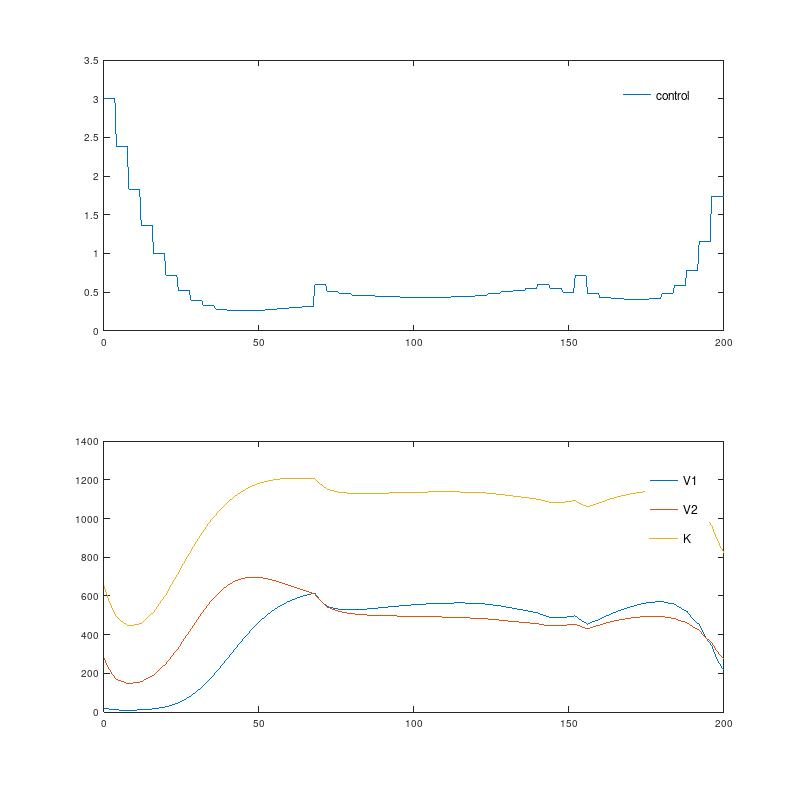
\includegraphics[width=\textwidth]{../plots/plot_nograd}
  \end{subfigure}
  \begin{subfigure}{.5\textwidth}
    \caption{Rozwiązanie z liczeniem gradientu}\label{test_sol}
    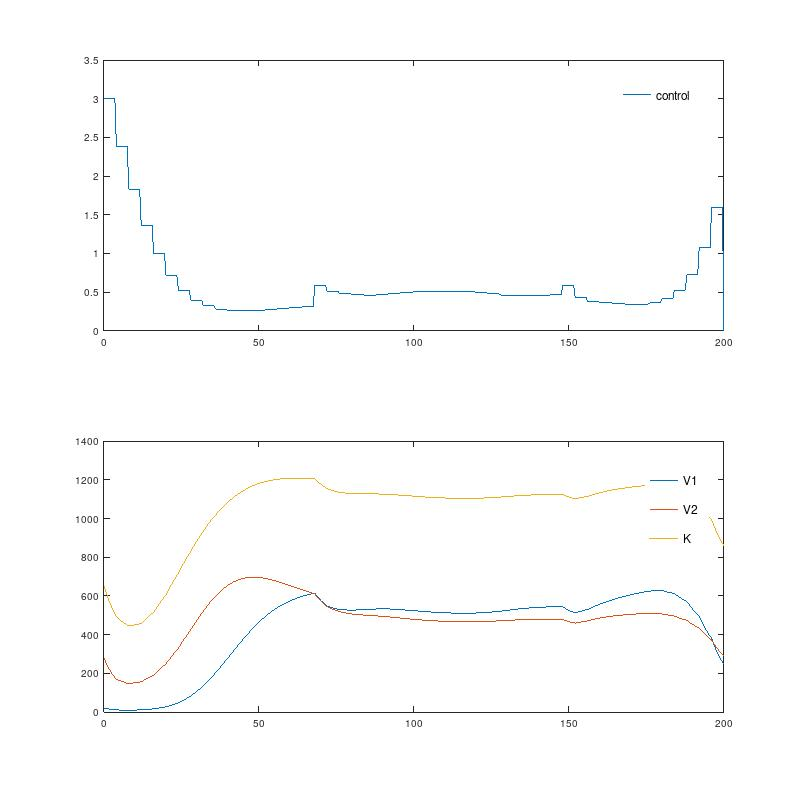
\includegraphics[width=\textwidth]{../plots/plot_test}
  \end{subfigure}%
  \caption{Rozwiązania dla przypadku testowego}\label{test_nograd_sol}
\end{figure}
Jak widzimy na Tabeli~\ref{test_tbl} i Rysunku~\ref{test_nograd_sol}, rozwiązania uzyskane obiema metodami są prawie identyczne, oraz nasza implementacja osiągnęła minimalnie lepszy wynik. Daje nam to dużą dozę pewności o poprawności naszej implementacji liczenia gradientu.

Warto tu jeszcze dodać, że liczba wywołań $\hat{J}$ podana na Tabeli~\ref{test_tbl} nie uwzględnia wywołań potrzebnych do oszacowania gradientu metodą różnic skończonych. Aby policzyć pochodną dla jednego parametru potrzeba raz dodatkowo wywołać $\hat{J}$, więc jednorazowe policzenie gradientu wymaga tylu wywołań ile jest parametrów (w tym przypadku 51). Gradient jest liczony w każdej iteracji co daje łącznie $20\cdot 51 = 1020$ dodatkowych wywołań $\hat{J}$. Inną wadą przybliżania gradientu metodą różnic skończonych są błędy numeryczne. Zauważmy, że w okolicy punktu przecięcia się krzywych $y_1$ i $y_2$ wartość i pochodna wyrażenia $G((y_2(t) - y_1(t))/\epsilon) = \frac{1 + \tanh(x)}{2}$ zmienia się bardzo szybko w czasie, co powoduje znaczne błędy przy zbyt dużym kroku metody różnic skończonych.

\subsubsection{Parametry 1.}
\begin{table}[h]
  \begin{center}
    \begin{tabular}{|c|c|c|c|c|c|c|c|c|}
      \hline
      Parametry & algorytm & dyskret. & siatka & $h$ & start & wynik & \#iteracji & \#wywołań $\hat{J}$ \\
      \hline
      1. & {\it lm\/} & stała & $S_1$ & 0.1 & $g_0$ & 2.2 & 3 & 8 \\
      \hline
      1. & {\it lm\/} & stała & $S_1$ & 0.1 & $g_3$ & 2.14 & 1 & 2 \\
      \hline
      1. & {\it lm\/} & stała & $S_{0.5}$ & 0.1 & $g_0$ & 2.19 & 3 & 8 \\
      \hline
      1. & {\it lm\/} & stała & $S_{0.5}$ & 0.1 & $g_3$ & 2.14 & 1 & 2 \\
      \hline
      1. & {\it lm\/} & stała & $N_{kon}$ & 0.1 & $g_0$ & 2.64 & 9 & 14 \\
      \hline
      1. & {\it lm\/} & stała & $N_{kon}$ & 0.1 & $g_3$ & 2.14 & 1 & 2 \\
      \hline
      1. & {\it lm\/} & liniowa & $S_1$ & 0.1 & $g_0$ & 2.21 & 2 & 7 \\
      \hline
      1. & {\it lm\/} & liniowa & $S_1$ & 0.1 & $g_3$ & 2.14 & 1 & 2 \\
      \hline
      1. & {\it lm\/} & liniowa & $S_{0.5}$ & 0.1 & $g_0$ & 2.21 & 2 & 7 \\
      \hline
      1. & {\it lm\/} & liniowa & $S_{0.5}$ & 0.1 & $g_3$ & 2.14 & 1 & 2 \\
      \hline
      1. & {\it lm\/} & liniowa & $N_{kon}$ & 0.1 & $g_0$ & 2.66 & 2 & 7 \\
      \hline
      1. & {\it lm\/} & liniowa & $N_{kon}$ & 0.1 & $g_3$ & 2.14 & 1 & 2 \\
      \hline
    \end{tabular}
    \caption{Eksperymetry z parametrami 1.}\label{param1_tbl}
  \end{center}
\end{table}

Przypadek ten okazał się mniej skomplikowany od Parametrów 2., więc poświęcimy mu tylko jeden eksperyment.

\subsubsection{Metoda dyskretyzacji}

%h - the place, b - bottom, t - top 
\begin{figure}[h]
%  \centering
  \begin{subfigure}{.5\textwidth}
%    \centering
    \caption{Rozwiązanie dla parametrów (\ref{exp1})}\label{max_sol}
    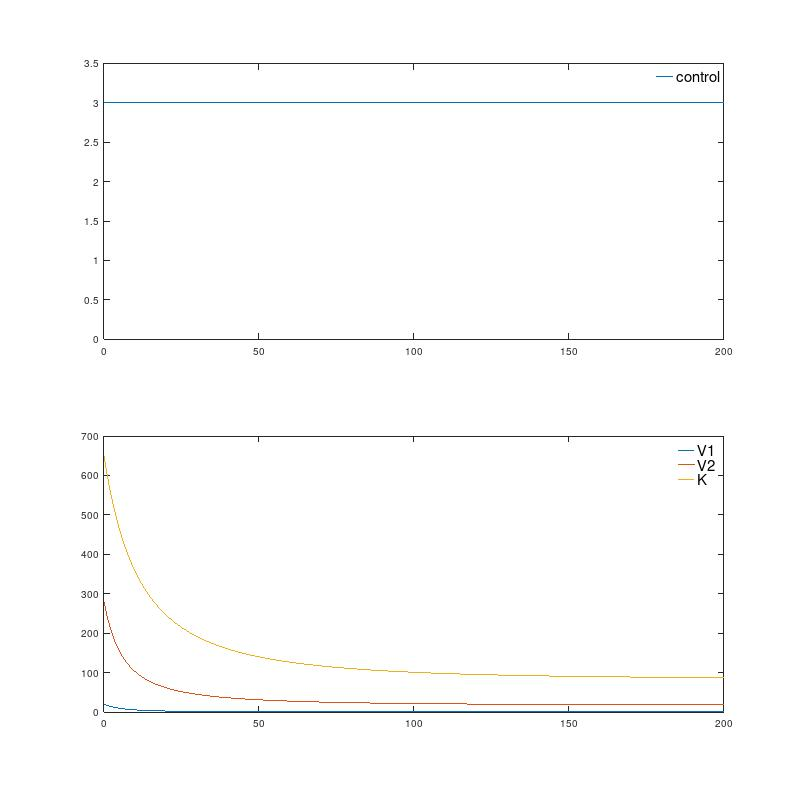
\includegraphics[width=\textwidth]{../plots/plot_max}
  \end{subfigure}
    \begin{subfigure}{.5\textwidth}
%    \centering
    \caption{Rozwiązanie dla parametrów (\ref{exp2})}\label{bang_sol}
    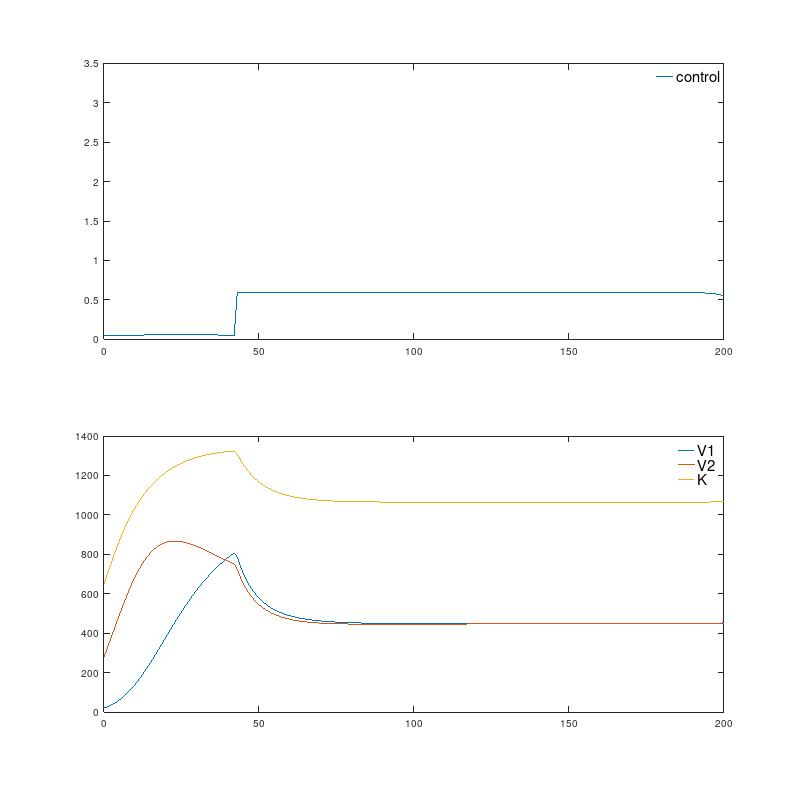
\includegraphics[width=\textwidth]{../plots/plot_bang}
  \end{subfigure}%
  \caption{Rozwiązania równania (\ref{ode})}\label{ode_sol}
\end{figure}

Dla parametrów (\ref{exp1}) wyniki eksperymentów są zgodne: najlepsze rezultaty osiągamy dla sterowania stale równego $g_{\max}$. Optymalizator zaczynając w nim nie znajduje żadnego lepszego punktu, natomiast dla wielu innych punktów startowych (n.p.\ dla sterowania stałego równego $0$ lub $1$) zbiega do sterowania niewiele różniącego się od stale równego $g_{\max}$. Stosowanie różnych algorytmów, siatek optymalizacji oraz metod przybliżania sterowania nie pozwoliło znaleźć istotnie różnego rozwiązania dającego obiecujące wyniki. Żaden eksperyment nie zbiegł do punktu dającego mniejszą wartość przybliżonego funkcjonału celu.

Wartość przybliżonego funkcjonału celu dla sterowania stale równego $g_{\max}$ to ok. $213575,7$. Dla porównania wartość przy braku leczenia, czyli sterowaniu stale równemu $0$, to ok. $567688,3$. Przybliżone rozwiązania równania (\ref{odesim}) przedstawiono na rysunku~\ref{max_sol}.

Dla parametrów (\ref{exp2}) wyniki są zauważalnie inne. Sterowanie stale maksymalnie nie osiąga już dobrych rezultatów (wynik to $407071.7$), natomiast najlepsze wyniki osiąga sterowanie mające na początku przedziału wartość ok. $0.05$, a w pozostałych punktach wartość ok. $0.59$. Funkcjonał celu dla tego sterowania osiąga wartość $272466.2$. Warto jeszcze dodać, że przy tych wartościach parametrów wyniki nie były tak zgodne, w trakcie eksperymentów znaleziono wiele rozwiązań o niewiele gorszych wynikach, niektóre z nich istotnie różne od przedstawionego. Przykład takiego rozwiązania zaprezentowano na rysunku \ref{weird_sol}. Wartość funkcjonału celu dla tego rozwiązania to $295794.6$, co jest o $8,6\%$ większe od rozwiązania optymalnego.

%\begin{figure}[h]
%  \centering
%  \caption{Nietypowe rozwiązanie dla parametrów (\ref{exp2})}\label{weird_sol}
%  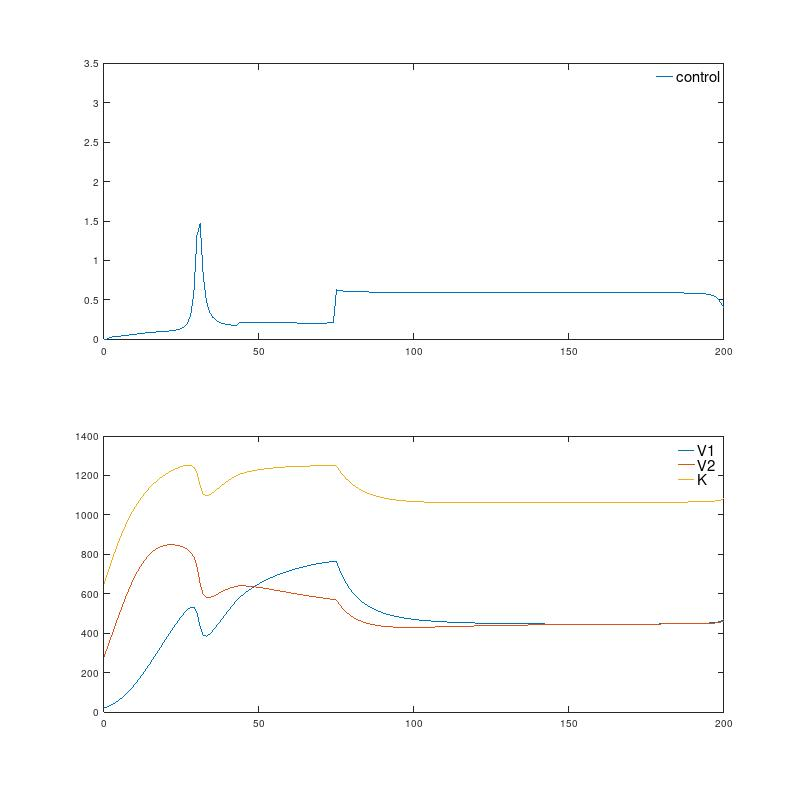
\includegraphics[width=.5\textwidth]{../plots/plot_weird}
%\end{figure}

%TODO zrobić optmalizację wzgl. punktu nieciągłości i wartości przed i po
\subsection{Analiza zastosowanych metod}

\begin{table}[h]
  \begin{center}
    \begin{tabular}{|c|c|c|c|c|c|}
      \hline
      & backend & start & wynik & \#iteracji & \#wywołań $\hat{J}$ \\
      \hline
      \multirow{3}{5em}{Parametry (\ref{exp1})} & {\it lm\_feasible\/} & $g(t) = 0$ & 234437.6 & 6 & 15 \\
      \cline{2-6}
      & {\it lm\_feasible\/} & $g(t) = g_{max}$ & 213575.7 & 1 & 2 \\
      \cline{2-6}
      & {\it sqp\/} & $g(t) = 0$ & 213575.7 & 8 & 9 \\
      \hline
      \multirow{5}{5em}{Parametry (\ref{exp2})} & {\it lm\_feasible\/} & $g(t) = 0$ & 324132.9 & 7 & 17 \\
      \cline{2-6}
      & {\it lm\_feasible\/} & $g(t) = 0.4\cdot\1_{[42.5,200]}$ & 283519.9 & 10 & 26 \\
      \cline{2-6}
      & {\it lm\_feasible\/} & $g(t) = 0.55\cdot\1_{[42.5,200]}$ & 272466.2 & 19 & 42 \\
      \cline{2-6}
      & {\it sqp\/} & $g(t) = 0$ & 340595.9 & 3 & 57 \\
      \cline{2-6}
      & {\it sqp\/} & $g(t) = 0.55\cdot\1_{[42.5,200]}$ & 272502.7 & 7 & 110 \\
      \hline
      \multirow{3}{6em}{Parametry (\ref{exp2}), siatka niejednorodna} & {\it lm\_feasible\/} & $g(t) = 0$ & 295303.8 & 20 & 42 \\
      \cline{2-6}
      & {\it lm\_feasible\/} & $g(t) = 0.4\cdot\1_{[42.5,200]}$ & 277775.5 & 14 & 35 \\
      \cline{2-6}
      & {\it lm\_feasible\/} & $g(t) = 0.55\cdot\1_{[42.5,200]}$ & 272848.2 & 19 & 42 \\
      \cline{2-6}
      & {\it sqp\/} & $g(t) = 0$ & 348091.2 & 2 & 53 \\
      \hline
    \end{tabular}
  \end{center}
  \caption{Wyniki niektórych eksperymentów}\label{resulttab}
\end{table}


Osiągnięcie przedstawionych wyników wymagało przeprowadzenia wielu eksperymentów, przetestowania różnych backendów optymalizatora, siatek optymalizacji, sterowania kawałkami stałego lub liniowego i różnych punktów startowych.
Jak widzimy, dla różnych wartości parametrów (\ref{exp1}) lub (\ref{exp2}), wyniki mocno się różnią i każdy z tych zestawów parametrów wymagał różnego podejścia. Wspólne dla obu tych problemów było działanie siatki optymalizacji. W większości eksperymentów zastosowano siatkę jednorodną o kroku $0.5$. Dalsze próby zagęszczania tej siatki nie poprawiły wyników, a tylko zwiększyły czas wykonania. Próby użycia siatki niejednorodnej przynosiły gorsze rezultaty niż te z siatką jednorodną o podobnej liczbie punktów. Jednym z powodów gorszych wyników siatki niejednorodnej mogą być fakt, że optymalizator zwykle dla takich siatek zbiegał do rozwiązania mającego znaczną różnice wartości na przedziałach z różnymi długościami kroku, które nie występowały przy siatce jednorodnej.

Dla parametrów (\ref{exp1}) najskuteczniejszym backendem był {\it sqp\/} który zbiegł do najlepszego rozwiązania zaczynając od zerowego sterowania, w przeciwieństwie do {\it lm\_feasable\/} który osiągnął trochę gorszy wynik $234437.6$ (dla tego samego punktu startowego). Nie było tu znaczącej różnicy między sterowaniem kawałkami stałym a kawałkami liniowym. Używanie różnych punktów startowych nie przynosiło wyraźnych różnic, z wyjątkiem zaczynania ze sterowania stale maksymalnego, dla którego optymalizacja kończyła się w jednej iteracji.

Dla parametrów (\ref{exp2}) najtrudniej było dobrać odpowiedni punkt startowy i na znalezieniu odpowiedniego punktu startowego skupiła się większość eksperymentów. W tym przypadku backend {\it sqp\/} okazał się znacznie gorszy od {\it lm\_feasable}, za wyjątkiem punktu startowego będącego bardzo blisko najlepszego rozwiązania. Podobnie kawałkami liniowe osiągało gorsze wyniki od sterowania kawałkami stałego, co pewnie jest powodowane nieciągłością  najlepszego rozwiązania. Znalezienie dobrego punktu początkowego wymagało postawienia hipotezy, że na początku wartość sterowania powinna być niska, a później wyższa. Zaczynając z takich pozycji optymalizacja zbiegała do punktu podobnego do najlepszego sterowania i wystarczyło już tylko wyznaczyć metodą prób i błędów najlepszy punkt nieciągłości, ponieważ optymalizator zaczynając z nieciągłego sterowania nie zmieniał punktu nieciągłości.

W kontekście tempa zbieżności i czasu działania różnych metod najważniejszym elementem jest samodzielne liczenie pochodnej, co zmniejszyło czas działania wielokrotnie oraz znacząco poprawiło tępo zbieżności i wyniki optymalizatora. W eksperymentach korzystających z domyślnego algorytmu liczenia pochodnej za pomocą różnic skończonych, trzeba było używać siatki posiadającej 4 razy mniej punktów, a i tak czas działania był wielokrotnie gorszy. Z tego powodu nie przeprowadzono wielu takich eksperymentów i nie będziemy dalej rozważać tego podejścia. Wypada też wspomnieć, że backend {\it sqp\/} wymagał zauważalnie więcej wywołań funkcji celu i czasu aby zbiec niż {\it lm\_feasable}. Dalszy wpływ punktu startowego i metody na wyniki i czas zbieżności zaprezentowano na tabeli \ref{resulttab}.
  
\section{Analiza i krytyka wyników}

Jak widzimy wyniki dla różnych rodzajów parametrów znacznie się różnią. Dokładniejsze przyjrzenie się funkcjonałowi celu (\ref{objfsim}) pozwala wyjaśnić takie zjawisko. Jak widzimy parametr $\omega$ jest mnożony przez wartość drugiej całki. Zauważmy, że funkcja pod drugą całką jest gładkim przybliżeniem funkcji znaku wyrażenia $y_2(t) - y_1(t)$. W zestawie parametrów (\ref{exp2}) parametr $\omega$ jest znacznie większy niż w (\ref{exp1}), więc w tym przypadku druga całka ma większy wpływ na wynik funkcjonału. Jak przyjrzymy się rozwiązaniu z rysunku \ref{bang_sol}), widzimy, że punkt nieciągłości znajduje się od razu po przecięciu się krzywych $y_1$ i $y_2$, a po nim sterowanie ma taką wartość aby krzywe te były bardzo blisko siebie, ale przy zachowaniu $y_2(t) - y_1(t) < 0$. Wygląda więc na to, przy wartościach parametrów (\ref{exp2}) bardziej opłaca się utrzymywać stan $y_2(t) - y_1(t) < 0$, natomiast przy wartościach (\ref{exp1}) lepsze wyniki daje minimalizacja pierwszej całki, czyli pola pod $y_1 + y_2$. Możemy się też spodziewać, że wysokie wartości sterowania powodują zmniejszanie się zarówno $y_1$ jak i $y_2$, ale od pewnej wartości sterowania $y_1$ maleje szybciej niż $y_2$. Taka hipoteza zgadzałaby się z interpretacją $y_1$ i $y_2$ jako liczba komórek rakowych odpowiednio podatnych na działanie leku i odpornych na niego, a wartości sterowania jako dawki leku.

\subsection{Krytyka wyników}
Wszystkie wyniki które udało się osiągnąć są minimami lokalnymi. Wynika to z zastosowanych technologii. Wyniki backendu {\it lm\_feasible\/} były mocno zależne od punktu startowego, natomiast backend {\it sqp\/}, który powinien szukać rozwiązania bardziej globalnie, miał nie najlepszą skuteczność. Być może zastosowanie innych backendów optymalizacji nieliniowej umożliwiłoby szukanie rozwiązania w sposób mniej zależący od znalezienia dobrego punktu startowego.

Niejednorodna siatka dyskretyzacji jest metodą nierzadko pozwalającą na poprawę tępa zbieżności, ale nie udało się jej tu z sukcesem zastosować. Podobnie przybliżanie sterowania za pomocą splajnów wyższego rzędu mogłoby poprawić tępo zbieżności. Być może zastosowanie tych metod oraz automatyzacja procesu znajdowania siatki dyskretyzacji np. metodą zastosowaną w \cite{Rao-ph} pozwoliłaby uzyskać lepsze wyniki.

Przypomnijmy jeszcze uwagę z początku pracy, że gdy $y_1 = y_2 = 0$, lub $y_3 = 0$ to zadanie nie jest dobrze określone, a w przypadku gdy wartości te są bliskie zeru, mogą występować znaczne błędy numeryczne. W żadnym eksperymencie wartości $y_1$ ani $y_2$ nie były bliskie zeru. Minimalna wartość $y_3$ z rysunku \ref{max_sol} to $14.9$, więc i ta nie jest zbyt bliska 0. Okazuje się jednak, że przy parametrach (\ref{exp2}), w rozwiązaniu (\ref{odesim}) dla sterowania stale równego $g_{max}$ minimalna wartość $y_3$ wynosi ok. $0.02$, więc ten eksperyment może być obarczony istotnym błędem numerycznym.

\newpage{}
\bibliography{bibliography}{}
\bibliographystyle{abbrv}
\end{document}
